\subsection{8. Лемма о разрастании для автоматных языков. Примеры неавтоматных языков.}

\Lemma (о накачке (разрастании))

Пусть $L$ - автоматный язык, $|L| = \infty$. Тогда:
$$\exists P \ \forall w \in L: |w| > P \ (\exists x, y, z: w = xyz, |xy| \leq P, |y| \neq 0: \forall k \in \N: xy^kz \in L)$$

Идея доказательства: \\
1) Рассмотрим НКА с однобуквенными переходами $M$. \\
2) Взять $P = |Q|$ (количество состояний), найти первый "цикл".

Рассмотрим $w \in L: |w| > P$ => То по принципу Дирихле, найдётся  состояние $q$, которые мы посетили дважды. Образовался цикл ($w = xyz$):

\begin{figure}[h]
    \hspace{-4ex} \begin{minipage}[h]{1\linewidth}
    \center{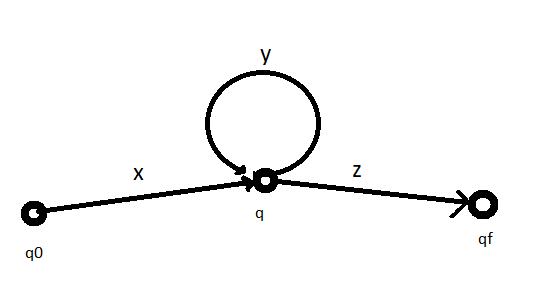
\includegraphics[width=0.45\linewidth]{1_7_1.png}}
    \end{minipage}
    \hspace{-4ex}
\end{figure}

\begin{enumerate}
    \item $|xy| \leqslant P = |Q|$: допустим, что $|xy| > P = |Q|$, тогда в $xy$ нашёлся бы цикл, где $q$ не будет являться первым пересечением;
    \item $|y| \neq 0$, так как среди переходов в автомате $M$ встречаются только однобуквенные, то существует хотя бы одно состояние $q_{new} \neq q$, которое будет посещено.
\end{enumerate}

Слово $xy^kz$ принадлежит языку $L$ для любого $k \in \N$, так как цикл, соответствующий $y$, может быть повторён $k$ раз. \EndProof

\Example Язык $\{ a^n b^n | n \in \N \}$ не является автоматным.

\Proof Воспользуемся отрицанием леммы о разрастании:
$$\forall p \ \exists w \in L : |w| \geqslant P \ \forall x, \ y, \ z: w = xyz, |xy| \leqslant P, \ |y| \neq 0: \forall k \in \N : xy^kz \notin L$$.
Возьмем произвольное $p$ и рассмотрим $w=a^pb^p$. Тогда 
$$w=xyz \,:\,\, |xy|\leqslant p, \,\,\, |y|\geqslant 0 \,\,\Rightarrow\,\, x = a^k, \,\, y=a^l, \,\, l > 0 \,\, \rightarrow\,\, z=a^{p-k-l}b^p$$
Рассмотрим $xy^2z = a^ka^{2l}a^{p-k-l}b^p = a^{p+l}b^p$. Так как $p+l \neq p$, значит $xy^2z \notin L$\,\,\, \EndProof